\documentclass[tikz,border=2]{standalone}
\usetikzlibrary{decorations.markings,shadows,arrows,shapes,positioning,calc,backgrounds,fit}
% Define the layers to draw the diagram
%
\newcommand{\vanish}[1]{}
%\newcommand{\vanish}[1]{#1}
\begin{document}
\pgfdeclarelayer{fg}
\pgfsetlayers{main,fg}
\definecolor{myBlue}{HTML}{1F77B4}
\definecolor{myRed}{HTML}{D62728}
%
\begin{tikzpicture}
[node distance=1cm,
bend angle=15,
subdue/.style={draw=black!30},
vertex/.style={draw=myBlue,shape=circle,inner sep=2pt},
seed/.style={shape=circle,draw=black,inner sep=2pt,fill=red},
infected/.style={shape=circle,draw=black,inner sep=2pt,fill=brown},
%
myedge/.style={semithick,black!50},
dedge/.style={semithick,black!50,dashed,>=latex', shorten >=.0pt, shorten <=.0pt},
vecArrow/.style={thick, decoration={markings,mark=at position 1 with
{\arrow[semithick]{open triangle 60}}}, double distance=2.5pt, shorten
>= 5.5pt, preaction = {decorate}, postaction = {draw,line width=1.4pt,
white,shorten >= 4.5pt}},
innerWhite/.style = {semithick, white,line width=1.4pt, shorten >= 4.5pt}]
%
%
\begin{scope}[xshift=0cm,yshift=0cm]
%%
\node (inf) at (0.5,1) {Original graph};
%%
\node (a1) [vertex] at (0,0) {\vanish{1}};
\node (a2) [vertex] at (-.5,-1){\vanish{2}};
\node (a9) [vertex] at (0.5,.5){\vanish{9}};
\node (a10) [vertex] at (0.7,-.5){\vanish{10}};

\node (a11) [vertex] at (1.2,-0.3){\vanish{11}};
\node (a12) [vertex] at (1.2,-.7){\vanish{12}};

\node (a3) [vertex] at (-.8,-2){\vanish{3}};
\begin{pgfonlayer}{fg}
\node (a14) [vertex] at (-.1,-1.7){\vanish{14}};
\end{pgfonlayer}
\node (a15) [vertex] at (-.2,-2.7){\vanish{15}};

\node (a4) [vertex] at (.5,-3){\vanish{4}};
\node (a16) [vertex] at (0.3,-3.4){\vanish{16}};
\node (a17) [vertex] at (0.7,-3.4){\vanish{17}};

\begin{pgfonlayer}{fg}
\node (a5) [vertex] at (.3,-1.3){\vanish{5}};
\node (a6) [vertex] at (.7,-2.2){\vanish{6}};
\node (a7) [vertex] at (1,-1.3){\vanish{7}};
\end{pgfonlayer}
\node (a8) [vertex] at (1.5,-2){\vanish{8}};

\node (a13) [vertex] at (2,-1.8){\vanish{13}};
\node (a18) [vertex] at (1.8,-2.5){\vanish{18}};
\node (a19) [vertex] at (2,-2.2){\vanish{19}};


%\node (a15) [vertex] at (2.2,-1){\vanish{15}};


\draw[myedge] (a1) -- (a2);
\draw[myedge] (a1) -- (a5);
\draw[myedge] (a1) -- (a9);
\draw[myedge] (a1) -- (a10);

\draw[myedge] (a2) -- (a3);
\draw[myedge] (a2) -- (a5);
\draw[myedge] (a2) -- (a14);

%\draw[myedge] (a3) -- (a4);
%\draw[myedge] (a3) -- (a6);
\draw[myedge] (a3) -- (a15);

\draw[myedge] (a4) -- (a6);
\draw[myedge] (a4) -- (a15);
\draw[myedge] (a4) -- (a14);
\draw[myedge] (a4) -- (a16);
\draw[myedge] (a4) -- (a17);

\draw[myedge] (a5) -- (a7);
\begin{pgfonlayer}{fg}
\draw[myedge] (a5) -- (a6);
%\draw[myedge] (a5) -- (a8);
%\draw[myedge] (a5) -- (a10);
%\draw[myedge] (a5) -- (a14);

\draw[myedge] (a6) -- (a7);
\draw[myedge] (a6) -- (a14); %node[midway,below] {$p$};
\end{pgfonlayer}

\draw[myedge] (a6) -- (a8);

\draw[myedge] (a7) -- (a8);
\draw[myedge] (a7) -- (a10);
\draw[myedge] (a7) -- (a14);

\draw[myedge] (a8) -- (a13);
\draw[myedge] (a8) -- (a18);
\draw[myedge] (a8) -- (a19);

\draw[myedge] (a10) -- (a11);
\draw[myedge] (a10) -- (a12);
\end{scope} 

\begin{scope}[xshift=2.5cm,yshift=-1.5cm]
\node (x1) at (-.25,0) {};
\node (x2) at (1.25,0) {};
\draw[vecArrow] (x1) -- (x2);
\node (inf) at (.5,1) {\parbox{2.2cm}{\centering \small add $n\epsilon$
random edges}};
\draw[innerWhite] (x1) -- (x2);
\end{scope}

%%%%%%%%%%%%%%%%%%%%%%%%%%%%%%%%%%%%%%%%%%%%%%%%%%%%%%%
% perturbed graph starts
%%%%%%%%%%%%%%%%%%%%%%%%%%%%%%%%%%%%%%%%%%%%%%%%%%%%%%%
\begin{scope}[xshift=5cm,yshift=0cm]
\node (a1) [vertex] at (0,0) {\vanish{1}};
\node (a2) [vertex] at (-.5,-1){\vanish{2}};
\node (a9) [vertex] at (0.5,.5){\vanish{9}};
\node (a10) [vertex] at (0.7,-.5){\vanish{10}};

\node (a11) [vertex] at (1.2,-0.3){\vanish{11}};
\node (a12) [vertex] at (1.2,-.7){\vanish{12}};

\node (a3) [vertex] at (-.8,-2){\vanish{3}};
\begin{pgfonlayer}{fg}
\node (a14) [vertex] at (-.1,-1.7){\vanish{14}};
\end{pgfonlayer}
\node (a15) [vertex] at (-.2,-2.7){\vanish{15}};

\node (a4) [vertex] at (.5,-3){\vanish{4}};
\node (a16) [vertex] at (0.3,-3.4){\vanish{16}};
\node (a17) [vertex] at (0.7,-3.4){\vanish{17}};

\begin{pgfonlayer}{fg}
\node (a5) [vertex] at (.3,-1.3){\vanish{5}};
\node (a6) [vertex] at (.7,-2.2){\vanish{6}};
\node (a7) [vertex] at (1,-1.3){\vanish{7}};
\end{pgfonlayer}
\node (a8) [vertex] at (1.5,-2){\vanish{8}};

\node (a13) [vertex] at (2,-1.8){\vanish{13}};
\node (a18) [vertex] at (1.8,-2.5){\vanish{18}};
\node (a19) [vertex] at (2,-2.2){\vanish{19}};

\draw[myedge] (a1) -- (a2);
\draw[myedge] (a1) -- (a5);
\draw[myedge] (a1) -- (a9);
\draw[myedge] (a1) -- (a10);

\draw[myedge] (a2) -- (a3);
\draw[myedge] (a2) -- (a5);
\draw[myedge] (a2) -- (a14);

%\draw[myedge] (a3) -- (a4);
%\draw[myedge] (a3) -- (a6);
\draw[myedge] (a3) -- (a15);

\draw[myedge] (a4) -- (a6);
\draw[myedge] (a4) -- (a15);
\draw[myedge] (a4) -- (a14);
\draw[myedge] (a4) -- (a16);
\draw[myedge] (a4) -- (a17);

\draw[myedge] (a5) -- (a7);
\begin{pgfonlayer}{fg}
\draw[myedge] (a5) -- (a6);
%\draw[myedge] (a5) -- (a8);
%\draw[myedge] (a5) -- (a10);
%\draw[myedge] (a5) -- (a14);

\draw[myedge] (a6) -- (a7);
\draw[myedge] (a6) -- (a14); %node[midway,below] {$p$};
\end{pgfonlayer}

\draw[myedge] (a6) -- (a8);

\draw[myedge] (a7) -- (a8);
\draw[myedge] (a7) -- (a10);
\draw[myedge] (a7) -- (a14);

\draw[myedge] (a8) -- (a13);
\draw[myedge] (a8) -- (a18);
\draw[myedge] (a8) -- (a19);

\draw[myedge] (a10) -- (a11);
\draw[myedge] (a10) -- (a12);
%%%%%
\draw[dedge] (a5) -- (a10);
\draw[dedge] (a8) -- (a14);
\draw[dedge] (a15) -- (a14);
\draw[dedge] (a6) -- (a18);
\draw[dedge] (a9) -- (a12);
\draw[dedge] (a18) -- (a19);
\end{scope}
%%%%
\begin{scope}[xshift=7.5cm,yshift=-1.5cm]
\node (x1) at (-.25,0) {};
\node (x2) at (1.25,0) {};
\draw[vecArrow] (x1) -- (x2);
\draw[innerWhite] (x1) -- (x2);
\node (inf) at (.5,1) {\parbox{2.2cm}{\centering \small Effect on IC model
}};
\end{scope}
\node[inner sep=0pt] at (12.25,-1.5) {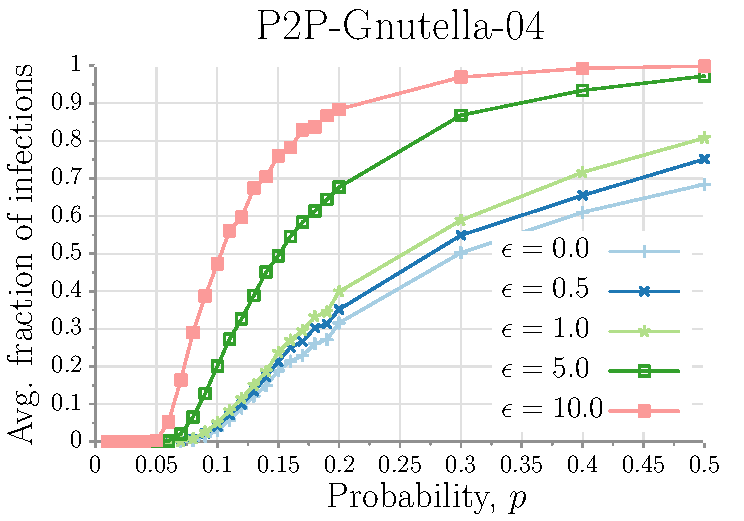
\includegraphics[width=.5\textwidth]{aux/p2p.pdf}};
%%%%
\end{tikzpicture}
\end{document}
